Let us now discuss the layout of the code and the files which are designed to be edited. The user is expected interact with 3 files \texttt{main.py}, \texttt{Settings.py} and \texttt{PlotterSettings.py}, these files along with a geometry file (\texttt{.geo} file) (see Section \ref{sect.geo}) allow the user to produce an array of different frequency sweeps for many different objects. In this section we discuss the layout of the folder system in place, how each of the input files can used and edited by the user to produce a frequency sweep along with how and where the results are saved. The structure of the code can be seen in Figure \ref{fig:FrequencySweepCode}
\begin{figure}[H]
\begin{center}
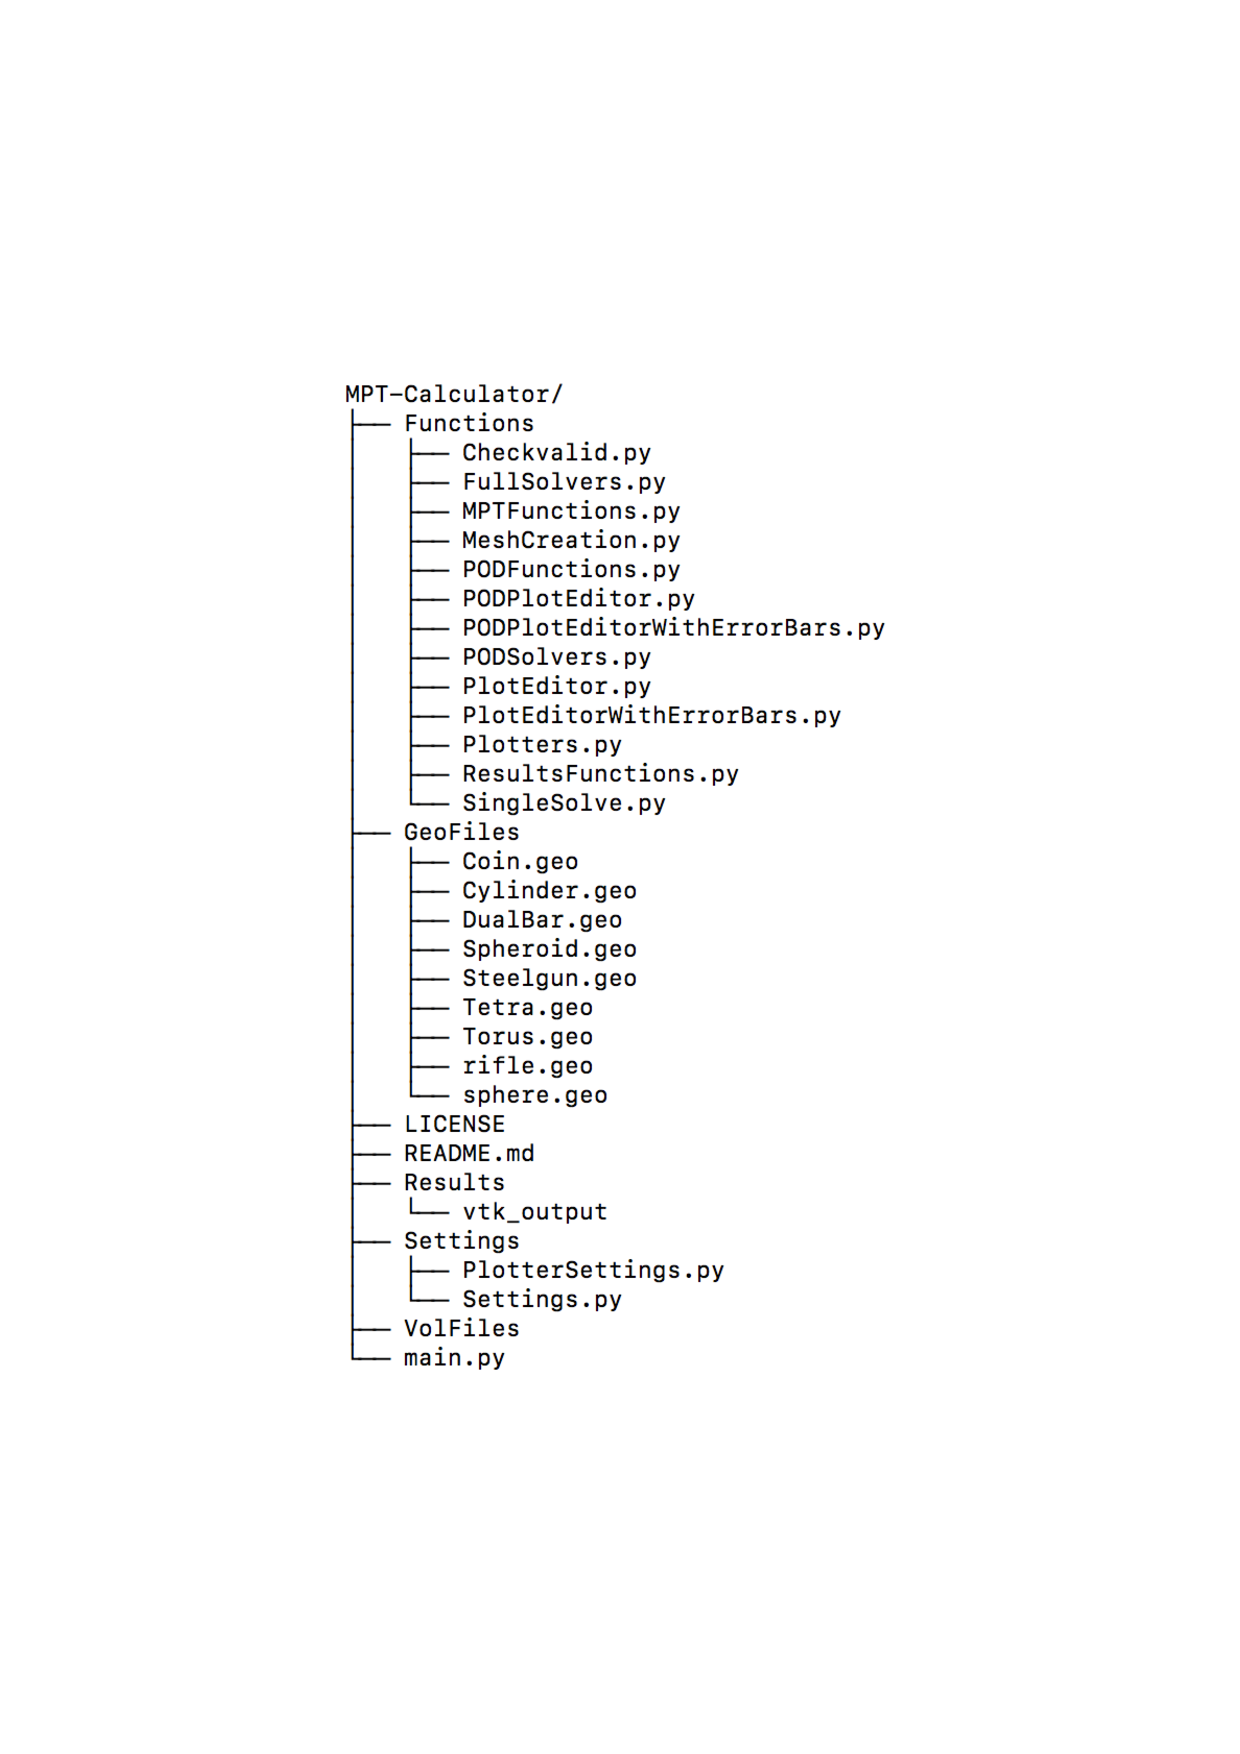
\includegraphics[width=0.4\textwidth]{Figures/CodeLayout}
\caption{Image displaying the structure of the main folder of the FrequencySweepCode.}\label{fig:FrequencySweepCode}
\end{center}
\end{figure}
\noindent
We next discuss how to use the input files of the code.\\
\subsection{User input files}
The files (along with their file paths) the user is expected to interact with are\\
\\
\texttt{main.py}\\
\texttt{Settings/Settings.py}\\
\texttt{Settings/PlotterSettings.py}.\\
\\
Once the files have the desired inputs the simulation is run by entering the command\\
\\
\texttt{python3 main.py}\\
\\
possibly replacing \texttt{python3} with \texttt{python3.8} here and throughout depending on your setup and version installed to the command line from the main directory. The \texttt{MPT-Calculator} then runs the appropriate frequency sweep and saves the outputs in an output folder (see Section \ref{sectOutput}).
We start this explanation with \texttt{main.py}.

\subsubsection{\texttt{main.py}}\label{sectmain.py}
The file \texttt{main.py} is the file with which the user is expected to have most interaction, it is the file which calls functions to generate a mesh, perform frequency sweeps and finally post process the data produced in the frequency sweep. In \texttt{main.py}, the user is greeted with an input section which should look similar to the image in Figure \ref{fig:main.py}.
\begin{figure}[H]
\begin{center}
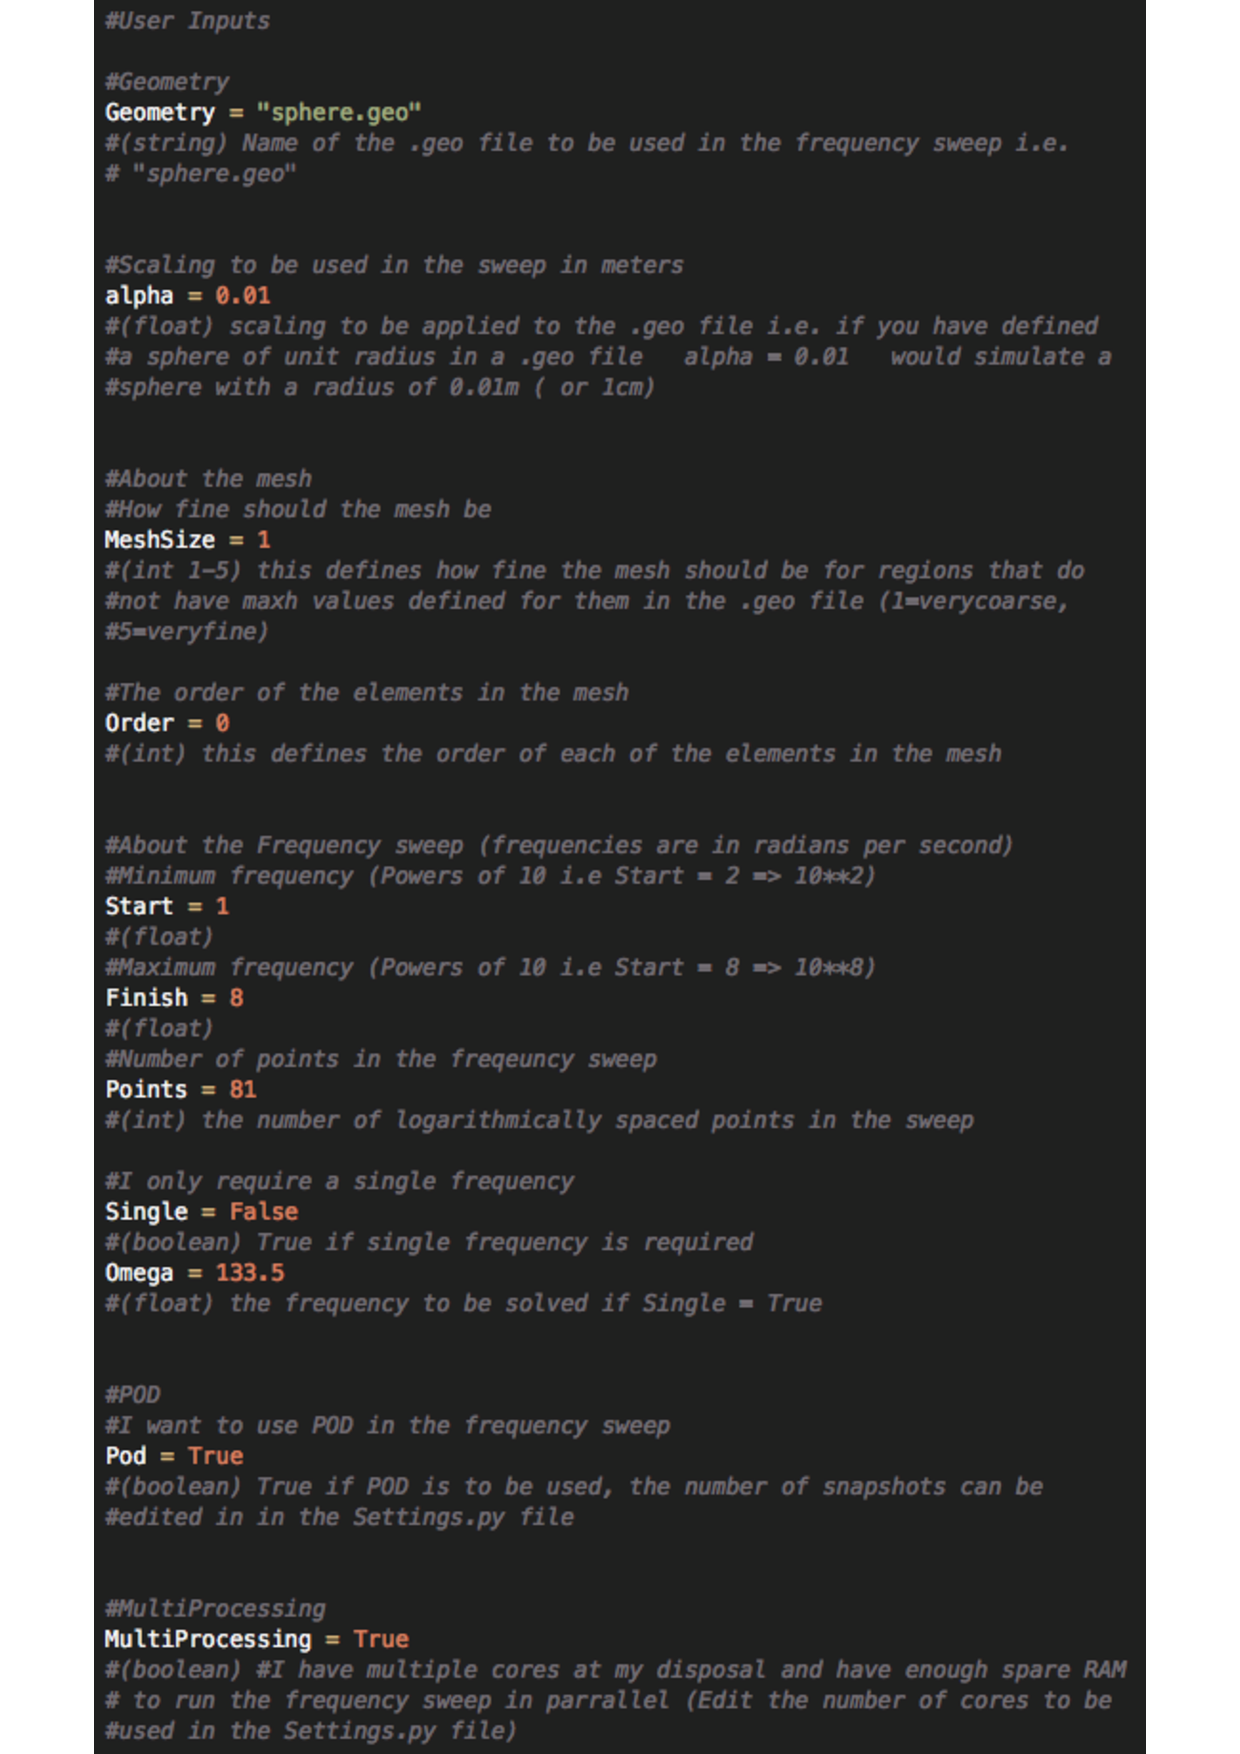
\includegraphics[width=0.8\textwidth]{Figures/mainpy.pdf}
\caption{Image displaying the user input section of the file \texttt{main.py}}\label{fig:main.py}
\end{center}
\end{figure}
\noindent
In this section we shall briefly explain what each of these inputs refer to and how to provide an input for each. For the first input \texttt{Geometry} the user is required to define the \texttt{.geo} (geometry) file which is to be used in the sweep see Section \ref{sect.geo} for information on how to create geometry files) this input is a string and can be defined as follows \\
\\
\texttt{Geometry = "sphere.geo"}\\
\\
A frequency sweep would then be calculated the object defined in file \texttt{sphere.geo}. The object defined in this file is then scaled by the parameter $\alpha$ (meters), the input for this is a float and can be defined as follows\\
\\
\texttt{alpha = 0.01}\\
\\
This then defines how the object in the \texttt{.geo} file should be scaled. The next two options in the file relate to the mesh which is to be used in the simulation of the object. The variable \texttt{MeshSize} defines how refined the mesh used in the simulation should be, the input for this variable is an integer between 1 and 5 (1 being very coarse and 5 being very fine) and can be defined as follows\\
\\
\texttt{MeshSize = 3}\\
\\
The other key option when it comes to defining a mesh is the order of the elements (how complex the functions describing the solution are) this requires an integer input which is between 0 and 3 (0 being the fastest to run the least accurate and 3 being the slowest by most accurate) when running full simulations (not small tests) it is recommended that an order of 3 be used, this can be defined as follows\\
\\
\texttt{Order = 3}\\
\\
The next 3 inputs relate to the frequencies in radians/sec which should be included in the frequency sweep they are as follows, \texttt{Start} and \texttt{Finish} are the minimum and maximum frequencies which should be included (float) and \texttt{Points} is the number of logarithmically spaced frequencies to be sampled at (integer), n.b. these are the powers base 10 of the frequencies i.e. we create a frequency sweep for $10^{\texttt{Start}}-10^{\texttt{Finish}}$ rad/s. For example if we defined the following\\
\\
\texttt{Start = 1}\\
\texttt{Finish = 8}\\
\texttt{Points = 8}\\
\\
We would run a frequency sweep for 8 logarithmically spaced points between $10^1$ and $10^8$ i.e. for the following frequencies
$$\omega = 10^1,10^2,10^3,10^4,10^5,10^6,10^7,10^8\textrm{ rad/s}.$$
Along with this there is also an option to run a simulation for a single frequency this may be done using the variable \texttt{Single} (boolean) and can be done as follows\\
\\
\texttt{Single $=$ True}\\
\\
This then runs a simulation at the the value defined for the variable \texttt{Omega} (float) n.b. this value is the frequency not the power of 10 of the frequency i.e. setting\\
\\
\texttt{Omega = 133.5}\\
\\
will run a simulation for $\omega=133.5$ rad/s not $\omega=10^{133.5}$ rad/s. If \texttt{Single = False} the frequency sweep will be run for the frequencies defined by \texttt{Start}, \texttt{Finish} and \texttt{Points}. Finally the user will find some options which affect how the frequency sweep will be produced. The first of these is whether or not to create a reduced order model (ROM) using the method of proper orthogonal decomposition (POD) the user may define whether to use this by editing the variable \texttt{POD} (boolean), if the user would like the frequency sweep to be produced using POD they set\\
\\
\texttt{POD = True}\\
\\
The POD works by producing a frequency sweep for a small number of frequencies (snapshots), it then uses the solutions to create an ROM which can then be used to produce a full frequency sweep containing many more points at a fraction of the computational cost. It is useful to note at this point that although POD works very well as the relative permeability $\mu_r$ of the object being simulated increases the POD becomes less accurate, see the spheroid example. This brings us to our final user input in the \texttt{main.py} file which is the variable \texttt{MultiProcessing} this option decides whether to produce the frequency sweep using multiple cores, by setting\\
\\
\texttt{MultiProcessing = True}\\
\\
The wall clock time will be reduced but the frequency sweep then requires more of the machines resources since it is running simulations on multiple cores. The default setting for the number of cores to be used is 2 but can be edited in the default settings section of \texttt{Settings.py}.
\\
\subsubsection{\texttt{Settings/Settings.py}}\label{sectSettings.py}
The second section which the users is able to interact with is the \texttt{Settings.py} file. This file contains settings related to how the frequency sweep is to be run, any addition outputs the user would like, how the data should be saved and how \texttt{NGSolve} solves each of the finite element problems. The file is subdivided into the following sections, \texttt{DefaultSettings}, \texttt{AdditionalOutputs}, \texttt{SaverSettings} and \texttt{SolverParameters}.\\
\\
\\
\noindent
We start by discussing the inputs in \texttt{DefaultSettings}, an image of the section can be seen in Figure \ref{fig:DefaultSettings.py}.
\begin{figure}[H]
\begin{center}
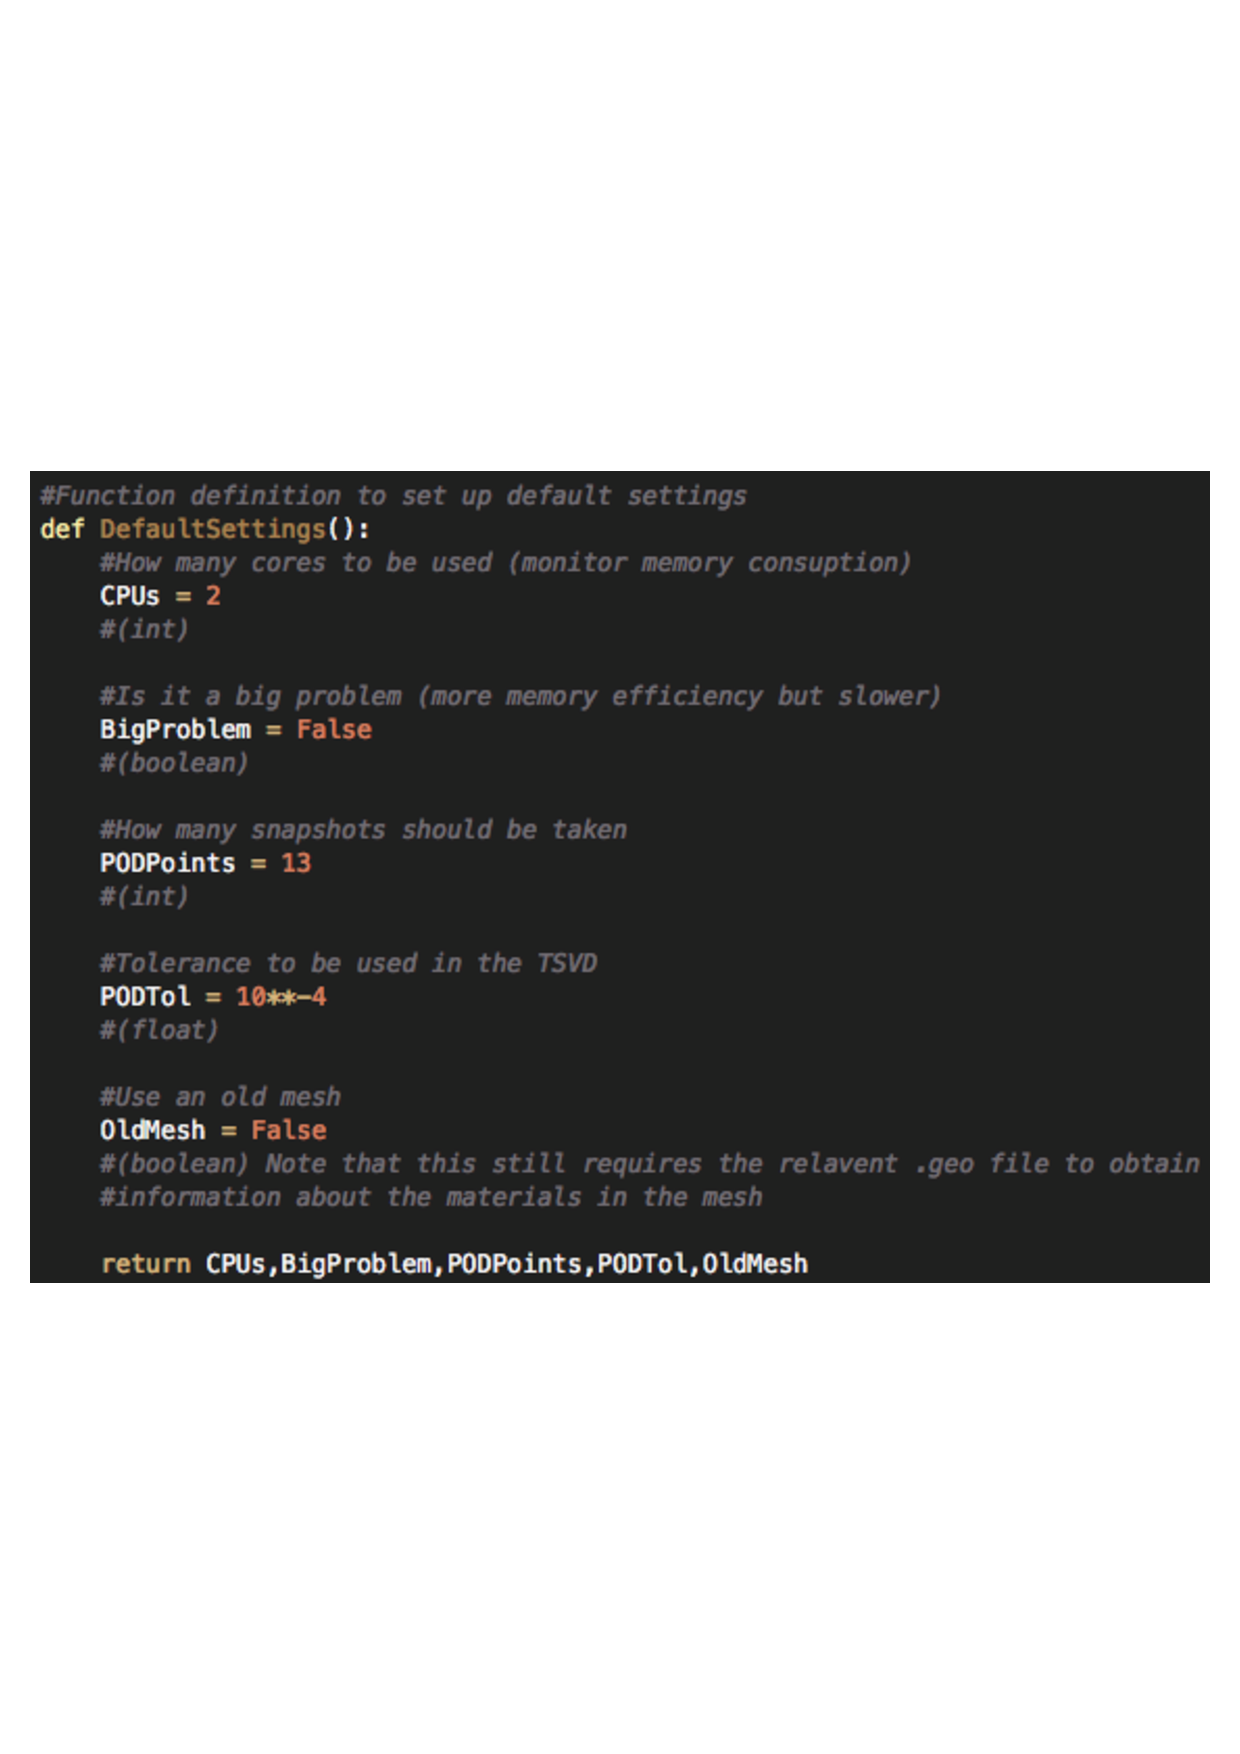
\includegraphics[width=0.7\textwidth]{Figures/DefaultSettings}
\caption{Image displaying the \texttt{DefaultSettings}}\label{fig:DefaultSettings.py}
\end{center}
\end{figure}
\noindent
This section defines variables relating about how to carry out the simulation. The number of cores is set by editing the variable \texttt{CPUs} (integer) an example of this would be setting\\
\\
\texttt{CPUs = 4}\\
\\
which would produce a frequency sweep using 4 of the machines cores. It is useful to mention at this point that when using multiple cores the user is recommended to monitor memory usage especially when producing a frequency sweep for an object with a fine mesh on a machine with limited resources. For larger problems, which are more memory intensive, we have an option for the simulation to use less memory (this option is for POD sweeps only). This is more memory efficient, however, it is both slower and effects performance of both the POD output and POD error bars. This option is engaged by editing the variable \texttt{BigProblem} (boolean), setting\\
\\
\texttt{BigProblem = True}\\
\\
This works by reducing the accuracy and therefore size of the snapshot solutions, saving each complex coefficient using the data type \texttt{np.complex64} (32-bit floats for both the real and imaginary parts). Although the use of this varies for different machines, for reference, using a 2015 mac with 8GB of ram it is advisable to set \texttt{BigProblem = True} for problem larger than 50,000 elements with $p=3$ with 13 snapshots or greater. The next two variables relate to the use of POD the first is \texttt{PODPoints} (integer), this defines how many snapshots should be taken when using the POD method, and can be set as\\
\\
\texttt{PODPoints = 13}\\
\\
This then creates an ROM using 13 snapshots (if \texttt{POD = True} in \texttt{main.py}). The other setting in the the \texttt{DefaultSettings} section is the variable \texttt{PODTol} (float) this variable sets at which point to truncate the singular value decomposition setting\\
\\
\texttt{PODTol = 10**-4}\\
\\
sets the truncation to the point at which the singular values drop below the $10^{-4}$ (for more explanation see~\cite{wilsonledger2019}). Suggested values for \texttt{PODPoints} and \texttt{PODTol} are 13 and $10^{-4}$ respectively. Lastly the setting \texttt{OldMesh} can be used to produce a frequency sweep with a precomputed mesh, saved in a \texttt{.vol} file. Since different versions of NGSolve produce different meshes this option allows you to run new examples using meshes produced on older versions of NGSolce. This is done by specifying the \texttt{.geo} file which contains the material information about the relevant mesh e.g. \texttt{Geometry = myshape.geo}, as well as supplying the \texttt{.vol} file e.g. \texttt{myshape.vol} to the \texttt{VolFiles} folder (this requires the \texttt{.geo} and \texttt{.vol} files to have the same name). Then by setting\\
\\
\texttt{OldMesh = True}\\
\\
the ``old mesh'' is used rather than producing a new mesh.\\
\\
\\
\noindent
Next we will discuss the section \texttt{AdditionalOutputs}, which defines the Additional outputs that the code returns, an image of the section can be seen in Figure \ref{fig:AdditionalOutputs.py}.
\begin{figure}[H]
\begin{center}
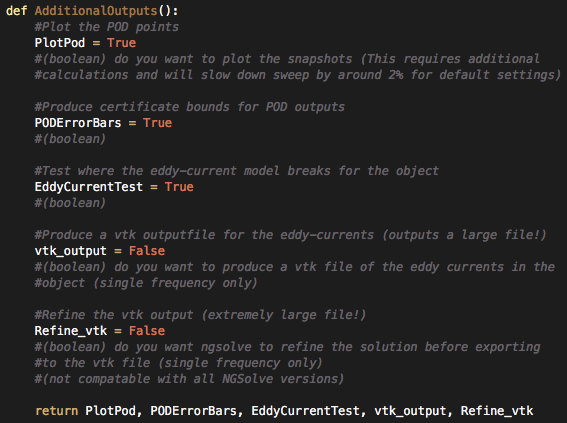
\includegraphics[width=0.7\textwidth]{Figures/AdditionalOutputs}
\caption{Image displaying the \texttt{AdditionalOutputs}}\label{fig:AdditionalOutputs.py}
\end{center}
\end{figure}
\noindent
The first variable \texttt{PlotPod} (boolean) defines whether or not to calculate and plot points where the POD has taken snapshots. These points can be plotted by setting\\
\\
\texttt{PlotPod = True}\\
\\
Having these points plotted can be very useful as it gives a visual representation of the accuracy of the frequency sweep produced by POD compared with a full order frequency sweep. We also give the user a way of producing the error certificates by editing the the variable \texttt{PODErrorBars} (boolean) which is selected by setting\\
\\
\texttt{PODErrorBars = True}\\
\\
This then produces error certificates for the POD outputs. The next option \texttt{EddyCurrentTest} (boolean) is to calculate the frequency at which the eddy current model is estimated to break down for the selected object, which may be lower than the prescribed maximum frequency and, for complex objects, may be a considerable restriction. Note this is based on a computation using the object's geometry rather than the standard engineering rules of thumb of saying the object is small compared to the wavelength and the conductivity is high  $\epsilon \omega < \sigma_*$ \cite{schmidt2008estimating}. This is selected by setting\\
\\
\texttt{EddyCurrentTest = True}\\
\\
These three outputs can be produced and saved then chosen to be shown or hidden after the sweep is run. The next two option are for the single frequency solve, with the solution of the single frequency problem the user may export the solution from NGSolve so that it can later be used by programs such as Paraview. This is done by editing the variables \texttt{vtk\_output} (boolean) and \texttt{Refine\_vtk} (boolean), by setting\\
\\
\texttt{vtk\_output = True}\\
\\
a \texttt{.vtk} file will be produced in the \texttt{vtk\_output} section of the \texttt{Results} folder, which contains the eddy-currents in the object. The user may also refine the solution before exporting by setting\\
\\
\texttt{Refine\_vtk = True}\\
\\
It is useful to take note at this point of the size of the files produced by these options an example is of a 2605 element mesh which when exported with no refinement produced a \texttt{.vtk} file of size 956 KB and with refinement produces a \texttt{.vtk} file of size 81.9 MB.\\
\\
\\
\noindent
We next discuss the section \texttt{SaverSettings}, this section allows the user to define a file path within the folder Results to save the outputs of the frequency sweep. An image of the section can be seen in Figure \ref{fig:SaverSettings.py}.
\begin{figure}[H]
\begin{center}
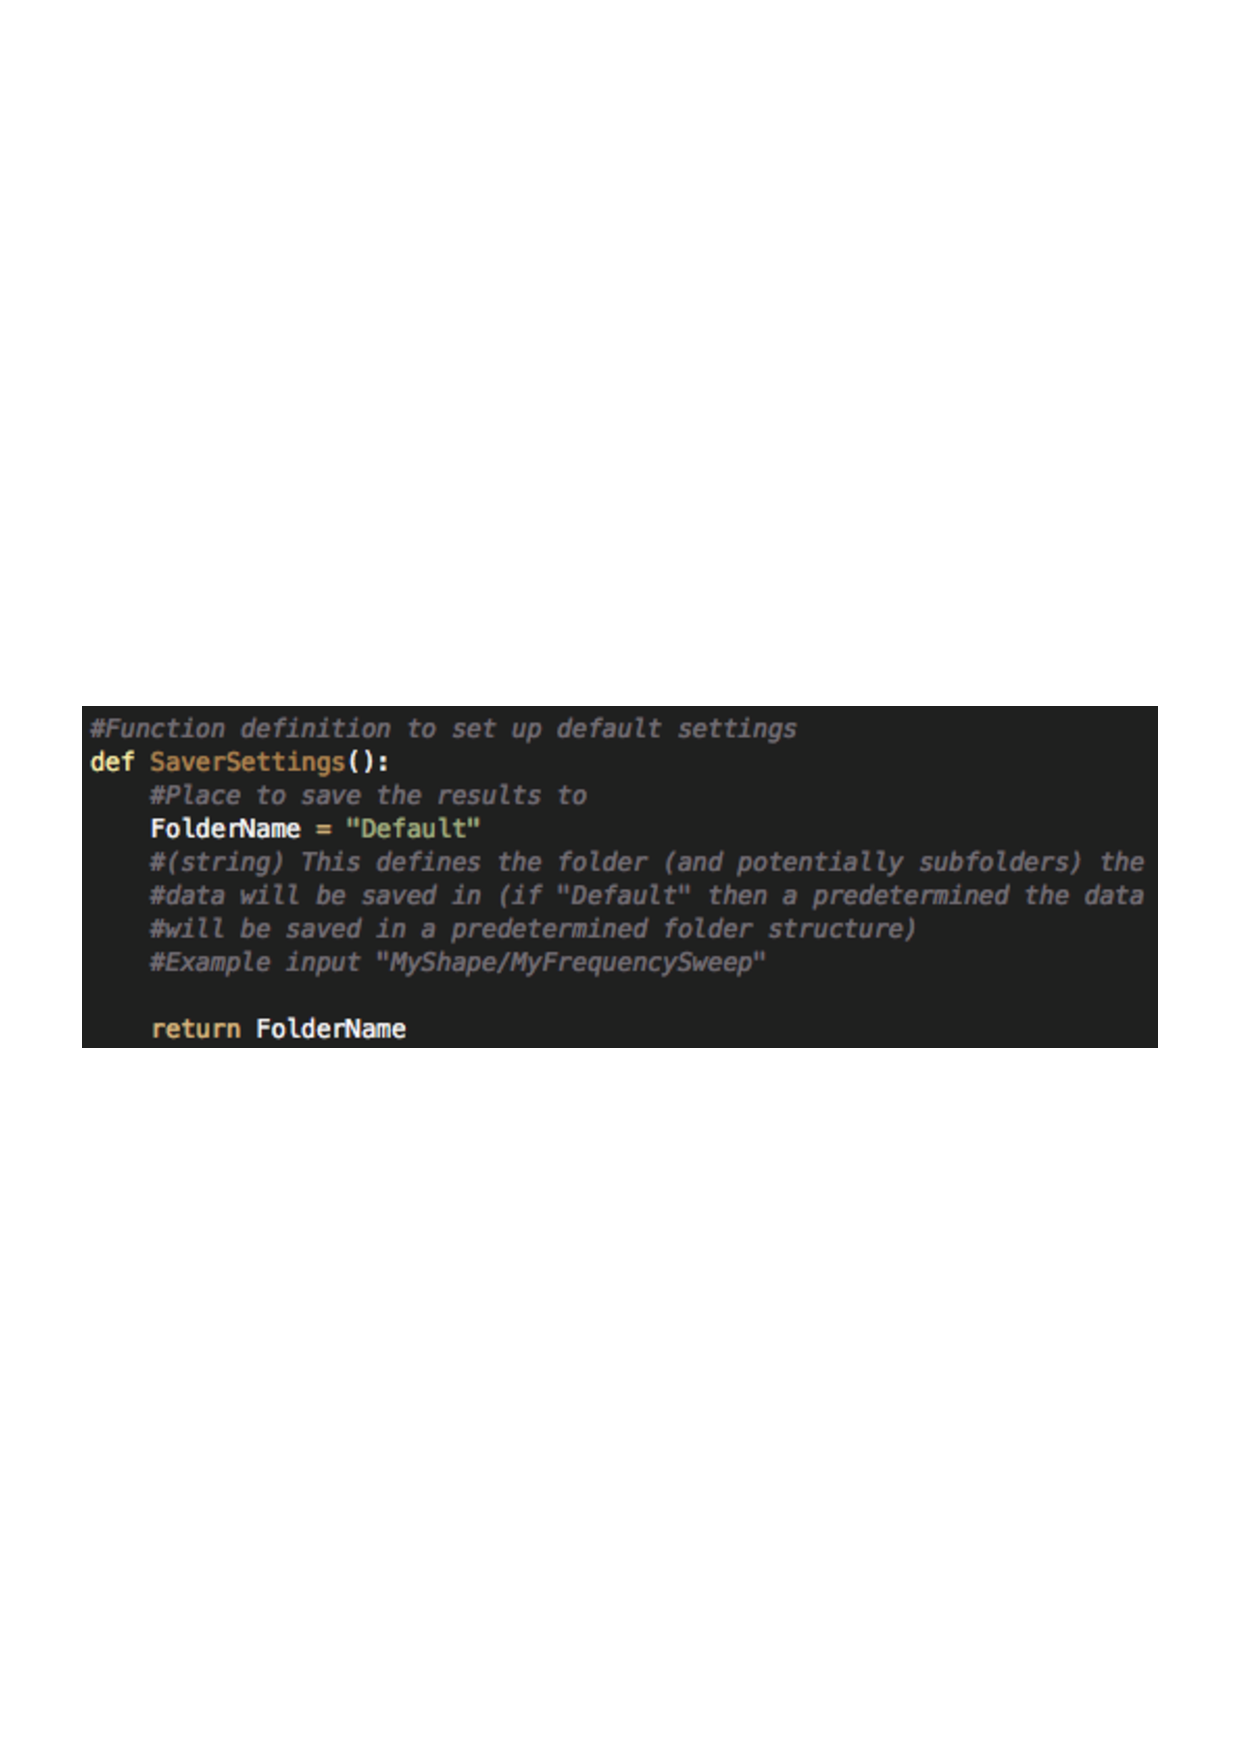
\includegraphics[width=0.7\textwidth]{Figures/SaverSettings}
\caption{Image displaying the \texttt{SaverSettings}}\label{fig:SaverSettings.py}
\end{center}
\end{figure}
\noindent
This is done by changing the variable \texttt{FolderName} (string) to the desired filepath within which save the outputs. An example of this would be\\
\\
\texttt{FolderName = MyShape/MyFrequencySweep}\\
\\
which would then store the output in \texttt{Results/MyShape/MyFrequencySweep}. Although this is an option, we recommend that \texttt{FolderName = "Default"}, which, when set, produces a series of subfolders containing information relating to material properties scaling and frequencies in the sweep. This makes it very hard for the user to overwrite (and lose) existing data from other frequency sweeps, which will be done if the user forgets to change \texttt{FolderName} for a new frequency sweep.\\
\\
\\
\noindent
The final section in \texttt{Settings.py} relates to how \texttt{NGSolve} solves each of the finite element problems. An image of this can be seen in Figure \ref{fig:SolverParameters.py}.
\begin{figure}[H]
\begin{center}
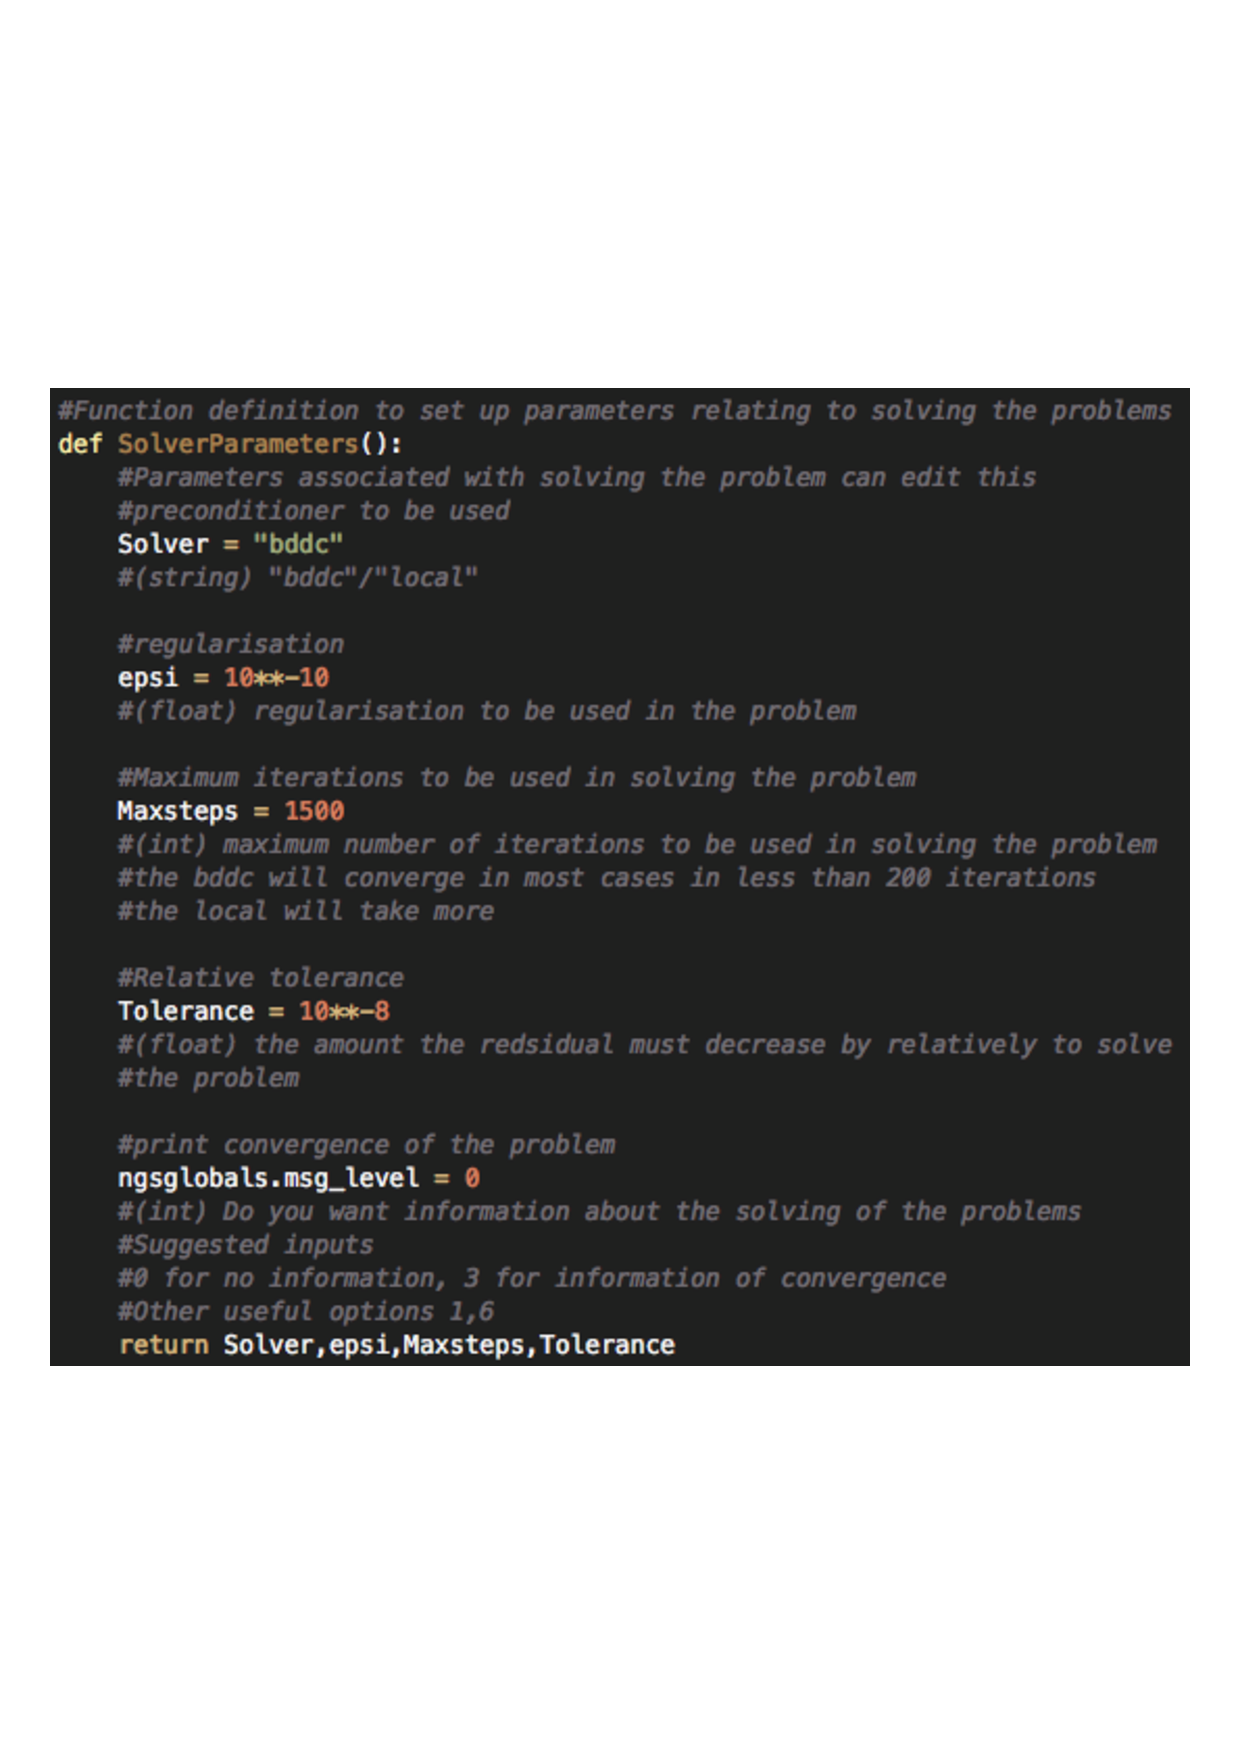
\includegraphics[width=0.7\textwidth]{Figures/SolverParameters}
\caption{Image displaying the \texttt{SolverParameters}}\label{fig:SolverParameters.py}
\end{center}
\end{figure}
\noindent
The default options work well for the frequency sweeps that are presented in the examples section. The default settings are as follows\\
\\
\texttt{Solver = "bddc"}\\
\\
\texttt{epsi = 10**-10}\\
\\
\texttt{Maxsteps = 1500}\\
\\
\texttt{Tolerance = 10**-8}\\
\\
\texttt{ngsglobals.msg\_level = 0}\\
\\
These settings are optimised for meshes containing more than 20,000, $3^{\textrm{rd}}$ order elements, see the examples section for further details. The options for the settings is as follows: The variable \texttt{Solver} (string) can be set to either \texttt{"bddc"} or \texttt{"local"} this changes the preconditioner used by the iterative CG solver in \texttt{NGSolve}. For simulations using very coarse meshes or simulations with $0^{\textrm{th}}$ order elements the \texttt{"local"} preconditioner is faster but for larger simulations setting\\
\\
\texttt{Solver = "bddc"}\\
\\
is recommended. The variable \texttt{tolerance} (float) sets the required relative residual for the iterative CG solver and controls the accuracy of the linear solve. For coarse discretisations, this does not need to be too small. For example, for  full order sweeps, setting\\
\\
\texttt{Tolerance = 10**-6}\\
\\
often leads to satisfactory results, however, upon testing, we found that for the POD the solution needs to be calculated more accurately to capture the underlying behaviour of the solution. The variables \texttt{epsi} (float) (regularisation) and \texttt{Maxsteps} (integer) (the maximum number of iterations performed) are less important since provided that \texttt{epsi} is 1 order of magnitude smaller than \texttt{tolerance} a solution will be reached within the maximum number of iterations. Finally, the variable \texttt{ngsglobals.msg\_level} (integer) relates to the information provided by \texttt{NGSolve} about solving the problems. We recommend that this be set to either \texttt{0} (for no information) or \texttt{3} (for information relating to the assembly and solving of the finite element problems). The next section explains how to use the \texttt{PlotterSettings.py} file.\\
\\
\subsubsection{\texttt{Settings/PlotterSettings.py}}\label{sectPlotterSettings.py}
To display the results of the frequency sweep a simple plotting function has been created\footnote{This is a basic visualisation tool, which allows the user to view results of the sweep. For a graph tailored to the users specification, use the data stored in the \texttt{.csv} files saved in the \texttt{Data} folder to produce their own plot.}, the settings of this function can be edited by changing the inputs of the \texttt{PlotterSettings.py} file. An image of the \texttt{PlotterSettings.py} file can be seen in Figure \ref{fig:PlotterSettings.py}. 
\begin{figure}[H]
\begin{center}
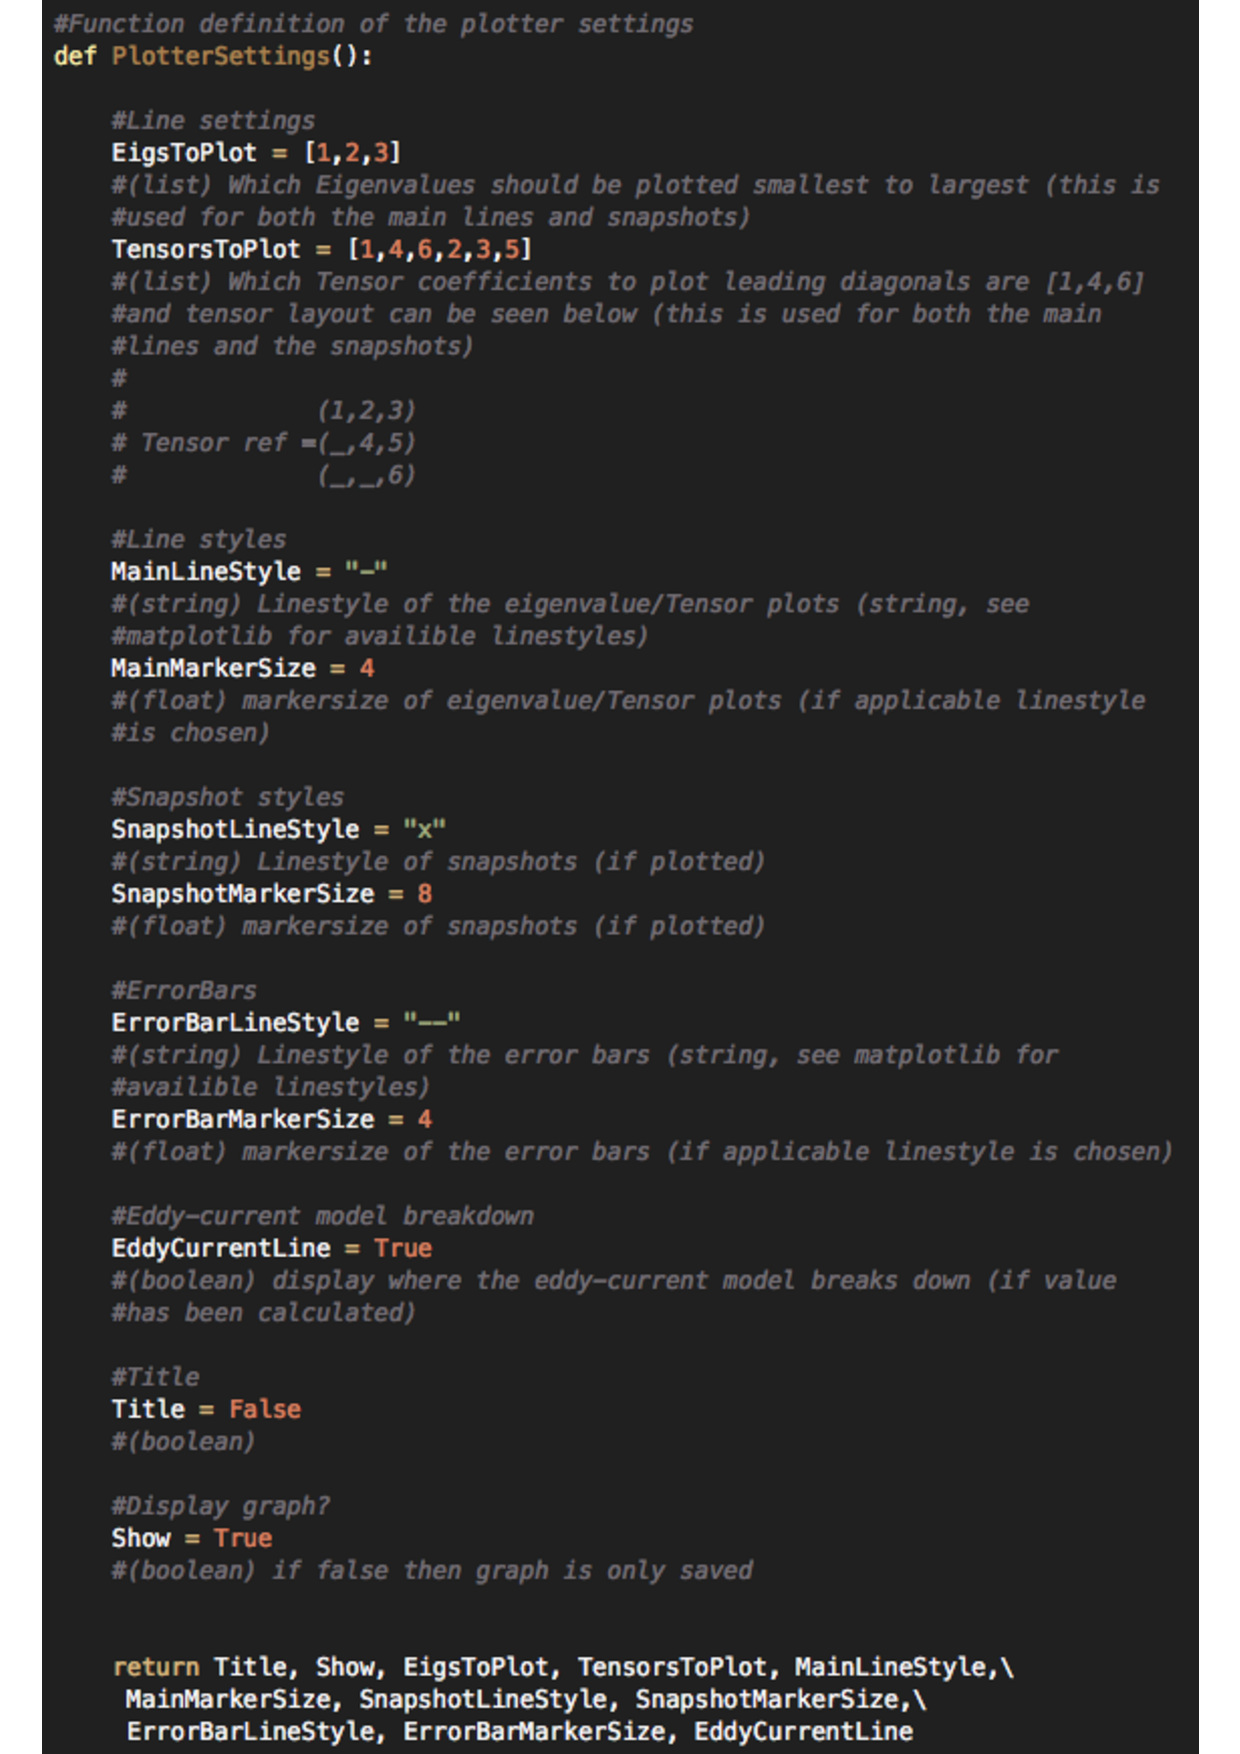
\includegraphics[width=0.8\textwidth]{Figures/PlotterSettingspy}
\caption{Image displaying the file \texttt{PlotterSettings.py}}\label{fig:PlotterSettings.py}
\end{center}
\end{figure}
\noindent
The first two inputs of the file \texttt{EigsToPlot} (list) and \texttt{TensorsToPlot} (list) relate to which lines are to be plotted on the graphs. With these options the user may change both the lines and the order in which the lines are to be plotted. The variable \texttt{EigsToPlot} defines which eigenvalues, sorted smallest to largest, are plotted. For example, setting\\
\\
\texttt{EigsToPlot = [3,2,1]}\\
\\
will plot all of the eigenvalues largest to smallest. The variable \texttt{TensorsToPlot} allows the user to choose which  coefficients of $\mathcal{M}$ are to be plotted. Taking account of the symmetry of the tensor,  the user has a choice of 6 independent coefficients to plot as referenced by the numbers in the following matrix
\begin{align}
\textrm{reference matrix}=\left[\begin{array}{ccc}
1 & 2 & 3\\
2 & 4 & 5\\
3 & 5 & 6
\end{array}\right].
\end{align}
For example, we may plot just diagonal coefficients of the matrix by setting\\
\\
\texttt{TensorsToPlot = [1,4,6]}\\
\\
For simplicity, a legend is created automatically for each of the lines in the plot, without additional inputs required from the user. The next 6 variables relate the style of lines being plotted. The variables \texttt{MainLineStyle} (string), \texttt{SnapshotLineStyle} (string) and \texttt{ErrorBarLineStyle} (string) define the line styles of the full frequency sweep and the line styles of the snapshots and certificate bounds (if \texttt{PlotPod = True} and/ or \texttt{PODErrorBars = True}), respectively. The plots are created using the matplotlib module of python and, thus, the available line styles are those supported by matplotlib \cite{matplotlib}. The other variables relating to line style are \texttt{MainMarkerSize} (float), \texttt{SnapshotMarkerSize} (float) and \texttt{ErrorBarMarkerSize} (float), which define the size of the markers used in the plot for the full sweep, snapshots and certificate bounds, respectively. The recommended settings of these vary on the markers chosen, but the default settings for the line styles and markers are\\
\\
\texttt{MainLineStyle = "-"}
\\
\texttt{MainMarkerSize = 4}
\\
\texttt{SnapshotLineStyle = "x"}
\\
\texttt{SnapshotMarkerSize = 8}
\\
\texttt{ErrorBarLineStyle = "--"}
\\
\texttt{ErrorBarMarkerSize = 4}\\
\\
The next variable, \texttt{EddyCurrentLine} (boolean), defines whether or not to plot the point at which the eddy-current model breaks down. This can be enabled by setting\\
\\
\texttt{EddyCurrentLine = True}\\
\\
The next variable, \texttt{Title} (boolean), defines whether or not the plot includes a title and, again, the title is automatically created for each of the different plots with no user input required. The default setting is\\
\\
\texttt{Title = True}\\
\\
The final variable is \texttt{Show} (boolean), which defines whether or not to display the produced graphs once the frequency sweep is complete\footnote{The graphs are automatically saved this option is whether to display them as well.}. The default setting is\\
\\
\texttt{Show = True}\\
\\
With this we conclude the section on how to interact with each of the input files. We next discuss how and where the output of the code is saved.\\

\subsection{Output files}\label{sectOutput}
In this section, we discuss how the outputs for each of the different versions of the code are saved. As mentioned briefly in Section~\ref{sectSettings.py}, the user may define which folder (or filepath) the outputs are saved in. However, when the code is run, it will generate subfolders to organise the results below this folder (or filepath), as described below. We start with the case of a single frequency simulation.\\


\subsubsection{Single frequency output}
In the case of a simulation with only one frequency, there is no need for a graphical representation, due to this the output folder has the structure shown in Figure \ref{fig:SingleOutput}.
\begin{figure}[H]
\begin{center}
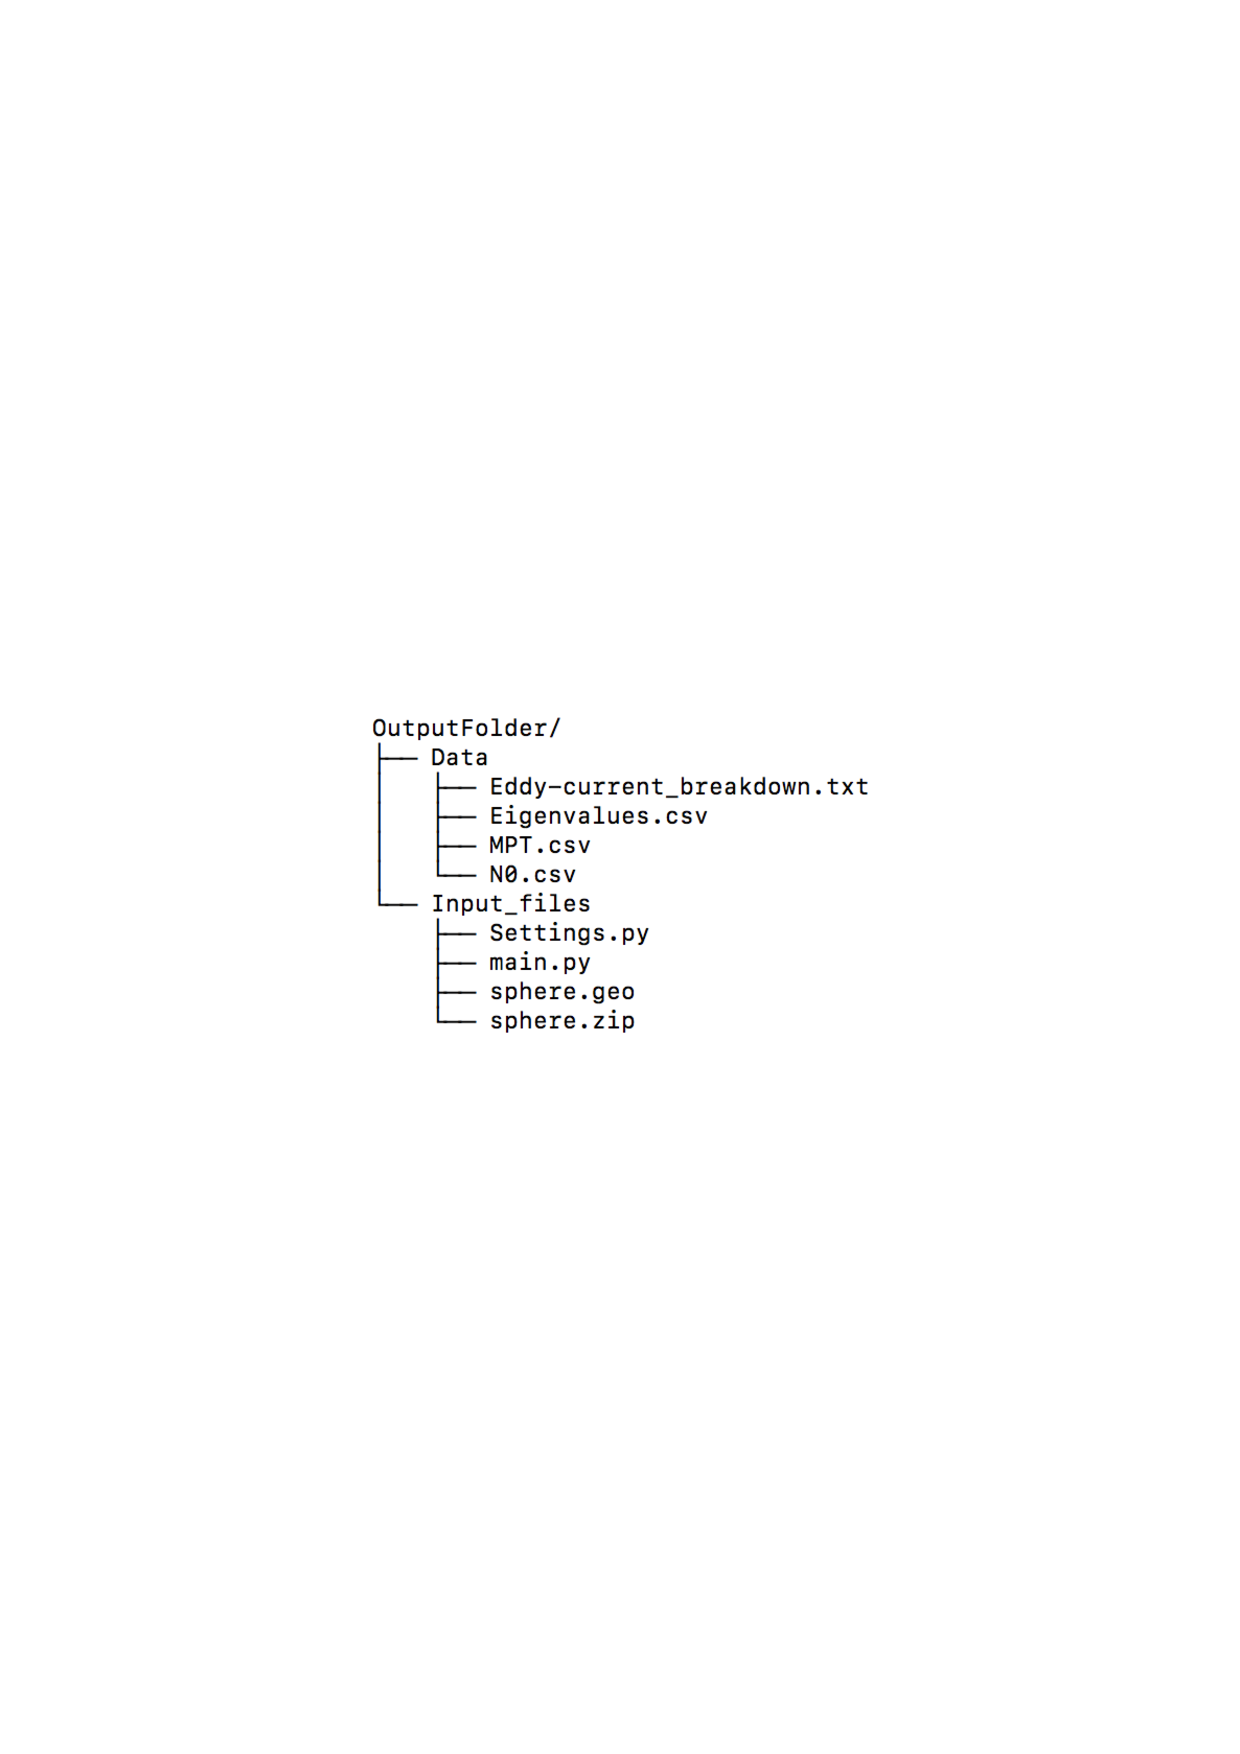
\includegraphics[width=0.3\textwidth]{Figures/SingleOutput}
\caption{Image displaying the structure of the output folder for the case of a single frequency simulation.}\label{fig:SingleOutput}
\end{center}
\end{figure}
\noindent
Notice the inclusion of the folder \texttt{Input\_files}, this folder contains a copy of the inputs files used to run the simulation. This allows the user to reproduce their results, if they so wish. We note the inclusion of the \texttt{sphere.zip} file which is a compressed version of the mesh used for the simulation (\texttt{sphere.vol} file).The folder \texttt{Data}, contains the results for the computed $\mathcal{M}$, $\mathcal{N}^0$, stored in \texttt{MPT.csv} and \texttt{N0.csv}, respectively,  and their eigenvalues $\lambda_i(\mathcal{N}^0+\mathcal{R})$ and $\lambda_i(\mathcal{I})$,  stored in the file \texttt{Eigenvalues.csv} as the sum $\lambda_i(\mathcal{N}^0+\mathcal{R})+\im\lambda_i(\mathcal{I})$ to reduce the number of output files. If the option \texttt{EddyCurrentTest = True} then we also have the \texttt{Eddy-current\_breakdown.txt} file, which states the frequency in rad/s at which the eddy current model breaks down.\\
\\
If the variable \texttt{vtk\_output = True}, we have the added output in the \texttt{vtk\_output} folder of the results folder which can be seen in Figure \ref{fig:VTKOutput}.
\begin{figure}[H]
\begin{center}
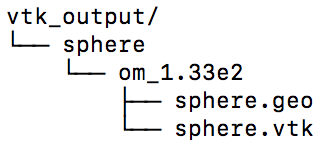
\includegraphics[width=0.22\textwidth]{Figures/vtkoutput}
\caption{Image displaying the structure of the output folder for the case of a single frequency simulation.}\label{fig:VTKOutput}
\end{center}
\end{figure}
\noindent
Here we store the \texttt{.vtk} file along with the associated \texttt{.geo} file which contains information about the materials used to construct the object. Let us next discuss the case of a full frequency sweep without using POD.\\

\subsubsection{Full order frequency sweep output}
In the case of the full order frequency sweep, the folder structure for the output folder can be seen in Figure \ref{fig:FullOrderOutput}.

\begin{figure}[H]
\begin{center}
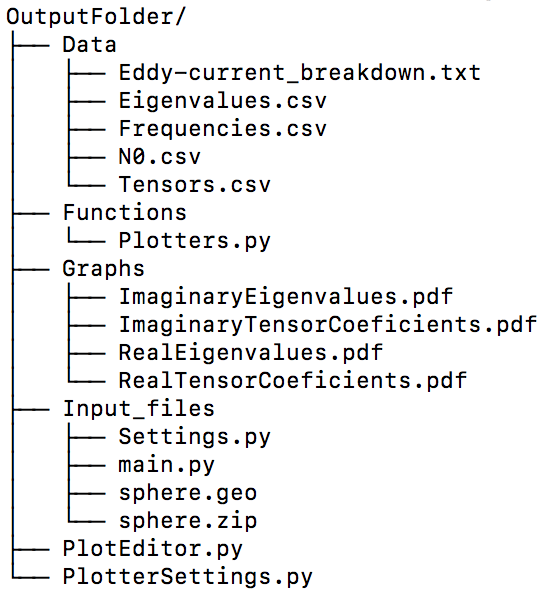
\includegraphics[width=0.35\textwidth]{Figures/FullOutput}
\caption{Image displaying the structure of the output folder for the full order frequency sweep.}\label{fig:FullOrderOutput}
\end{center}
\end{figure}
\noindent
The \texttt{Functions} folder contains the file \texttt{Plotters.py}, which contains the functions used for producing the plots. The folder \texttt{Graphs} contains the graphs displaying the results of the frequency sweep. The file \texttt{Frequencies.csv} contains a list of the frequencies for which the tensors have been calculated and  \texttt{Eigenvalues.csv} contains the sum  $\lambda_i(\mathcal{N}^0+\mathcal{R})+\im\lambda_i(\mathcal{I})$. The file \texttt{Tensors.csv} stores the MPTs coefficient as row vectors and stacks them so that each row corresponds to the same corresponding frequency in the row of the \texttt{Frequencies.csv} file and the eigenvalues in the row of the \texttt{Eigenvalues.csv} file. Finally, the files \texttt{PlotEditor.py} and \texttt{PlotterSettings.py}  allow the user to replot and edit the graphs by editing the inputs in \texttt{PlotterSettings.py} in the same manner as in \ref{sectPlotterSettings.py} and then running the file \texttt{PlotEditor.py}  by entering the command\\

\noindent \texttt{python3 PlotEditor.py}\\
\\
in the command line from the output folder. Next we discuss the case of a frequency sweep produced using POD.\\
\subsubsection{POD frequency sweep output}
In the case of a frequency sweep produced using POD there are two possible options for the structure of the output folder. If \texttt{PlotPod = True}, \texttt{PODErrorBars = True} and \texttt{EddyCurrentTest = True}, the folder will have the structure shown in Figure \ref{fig:PlotPodOutput}.
\begin{figure}[H]
\begin{center}
\includegraphics[width=0.35\textwidth]{Figures/PodOutput}
\caption{Image displaying the structure of the output folder for the frequency sweep using POD with the option of plotting the snapshot tensors.}\label{fig:PlotPodOutput}
\end{center}
\end{figure}
\noindent
The key differences to the full order solve are the inclusion of the data files \texttt{PODFrequencies.csv}, \texttt{PODEigenv\\alues.csv}, \texttt{PODTensors.csv} and \texttt{ErrorBars.csv}. These files contain the frequencies for the snapshots, the eigenvalues of the tensors calculated at the snapshots, the tensors calculated at the snapshots and the certificate bounds of the outputs, respectively. The other difference between this and the full order sweep is the inclusion of the extra plot editor files \texttt{PODPlotEditor.py}, \texttt{PODPlotEditorWithErrorBars.py} and \texttt{PlotEditorWithErrorBars.py}, which enables plots of both the snapshots and full frequency sweep to be reproduced.\\
\\
In the case where \texttt{PlotPod = False},  the structure is as shown in Figure \ref{fig:PlotPodOutput}  except that the files \texttt{PODEigenvalues.csv}, \texttt{PODTensors.csv} and \texttt{PODPlotEditor.py} are not included in the folder. Similarly when \texttt{PODErrorBars = False}, we find the exclusion of the files \texttt{ErrorBars.csv}, \texttt{PODPlotEditorWithError\\Bars.py} and \texttt{PlotEditorWithErrorBars.py} from the output folder. Finally when \texttt{PlotPod  = False} and \texttt{PlotEditorWithErrorBars.py = False} we have the exclusion of \texttt{PODEigenvalues.csv}, \texttt{PODTensors.csv} and \texttt{ErrorBars.csv} along with \texttt{PODPlotEditor.py}, \texttt{PODPlotEditorWithErrorBars.py} and \texttt{PlotEditorWi\\thErrorBars.py}.\\
\\
The user may replot the graphs by entering the commands\\

\noindent \texttt{python3 PlotEditorWithErrorBars.py}\\
\noindent \texttt{python3 PODPlotEditor.py}\\
\noindent \texttt{python3 PODPlotEditorWithErrorBars.py}\\
\\
in the output folder, to show a plot with the snapshots and/ or certificate bounds being displayed on the graph.  Or if the command\\

\noindent \texttt{python3 PlotEditor.py}\\
\\
is entered in the output folder, the graphs without the snapshots included is reproduced. With this we conclude our section on the overview and structure of the code. In the next section, we discuss how to create an object using a \texttt{.geo} file.\\





















